\documentclass{article}

\usepackage{mathrsfs,amsmath}
\usepackage{xcolor}
\usepackage{titlesec}
\usepackage{listings}
\usepackage{syntax}
\usepackage{pythonhighlighting}
\usepackage{graphicx}

\graphicspath{ {./assets/} }

\usepackage[margin=1.4in]{geometry}

\title{Handout \#11 | CS 471} 
\author{Jared Dyreson\\ 
        California State University, Fullerton}

\DeclareRobustCommand{\bowtie}{%
  \mathrel\triangleright\joinrel\mathrel\triangleleft}


\usepackage [english]{babel}
\usepackage [autostyle, english = american]{csquotes}
\MakeOuterQuote{"}

\titlespacing*{\section}
{0pt}{5.5ex plus 1ex minus .2ex}{4.3ex plus .2ex}
\titlespacing*{\subsection}
{0pt}{5.5ex plus 1ex minus .2ex}{4.3ex plus .2ex}

\usepackage{hyperref}
\hypersetup{
    colorlinks,
    citecolor=black,
    filecolor=black,
    linkcolor=black,
    urlcolor=black
}

\begin{document}

\maketitle
\tableofcontents

\newpage

\section{Questions}

\begin{enumerate}
\item What are the three major components of the SMTP protocol and it's role in the email delivery system?

\begin{itemize}
\item User agents
\item Mail servers
\item SMTP | Simple Mail Transfer Protocol
\end{itemize}

\item Explain the basic purpose of the SMTP protocol and it's role in the email delivery system

\begin{itemize}
\item SMTP spells out and directs how your email moves from your computer's MTA (Mail Transfer Agent) to an MTA on another computer
\end{itemize}

\item Explain the purpose of each SMTP command and the meaning of the response codes

\begin{figure}[!h]
\centering
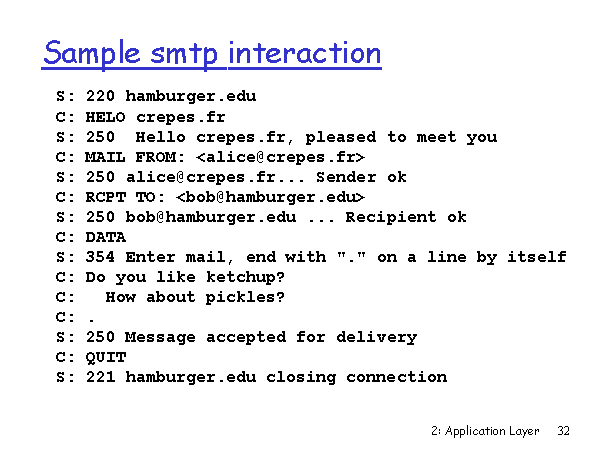
\includegraphics[width=10cm]{SMTP_Commands}
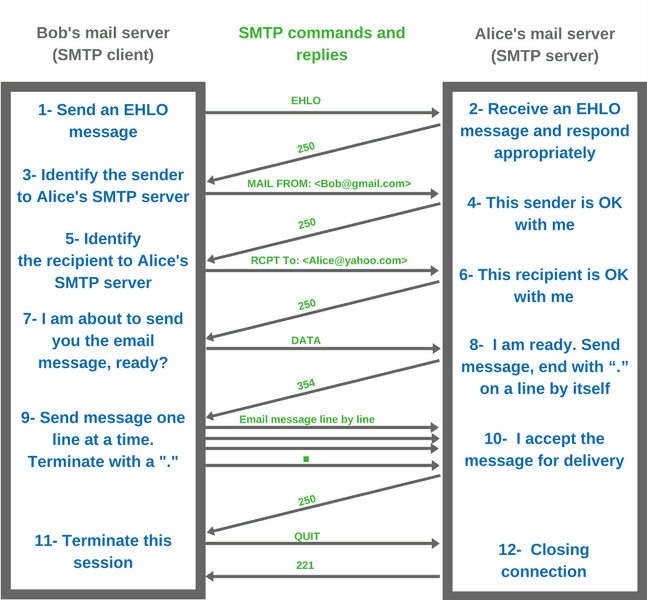
\includegraphics[width=6cm]{SMTP-sequence-diagram}
\end{figure}

\newpage

\item Give a sample sequence of command for sending an email using SMTP to your email address

\begin{verbatim}
S: 220 csu.fullerton.edu
C: HELO csu.fullerton.edu
S: 250
C: MAIL FROM: <professor@csu.fullerton.edu>
S: 250 .... sender ok
C: RCPT TO: <jareddyreson@csu.fullerton.edu>
S: 250 ....recipient ok
C: DATA
C: Did you do your homework?
C: .
S: 250 .... Message accepted
C: QUIT
S: 221  .... Closing connection
\end{verbatim}

\item Is SMTP a pull or push protocol?

\begin{itemize}
\item SMTP is a push protocol, it is only interested in moving along the information
\end{itemize}

\item Does SMTP use persistent or non-persistent connections?

\begin{itemize}
\item SMTP uses persistent connections, information must be passed through in a continuous stream
\end{itemize}

\item How does SMTP differ from HTTP

\begin{itemize}
\item \textbf{SMTP:}
\begin{itemize}
\item Is a push protocol
\item Persistent connection by default
\item Uses port 25
\item Places all objects into a single message
\end{itemize}
\item \textbf{HTTP:}
\begin{itemize}
\item Is a pull protocol
\item Can either be persistent or non-persistent
\item Uses port 80
\item Places each object in it's own HTTP message
\end{itemize}
\item More information can be found \href{https://www.educative.io/edpresso/smtp-vs-http}{\underline{here}}.
\end{itemize}

\newpage

\item What are the three different methods for retrieving email?

\begin{itemize}
\item POP: Post Office Protocol | authorization, download. The emails are immediately discarded when downloaded onto the host machine. However, there are ways to set a lifespan for emails, where they are deleted after a certain time frame.
\begin{figure}[!h]
\centering
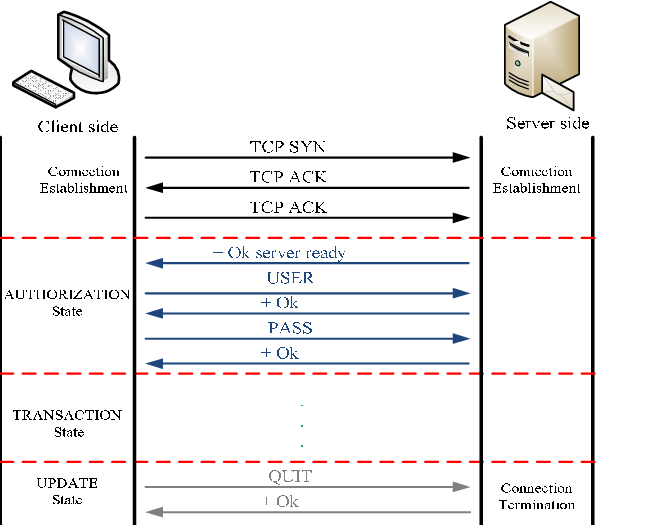
\includegraphics[width=10cm]{POP3-Client-Server-Procedure}
\caption{POP3 Protocol Example}
\end{figure}
\begin{figure}[!h]
\centering
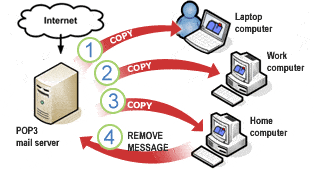
\includegraphics[width=7cm]{pop3_usage}
\caption{POP3 High Level View}
\end{figure}
\newpage
\item IMAP: Internet Mail Access Protocol | Most features, including manipulation of stored messages on server. 
\begin{itemize}
\item Provides more flexibility for managing emails stored on the mail server.
\item Think FTP
\item Keeps all messages in one place: the server
\item Allows for user to organize messages in folders
\item Keeps user state across sessions
\end{itemize}
\begin{figure}[!h]
\centering
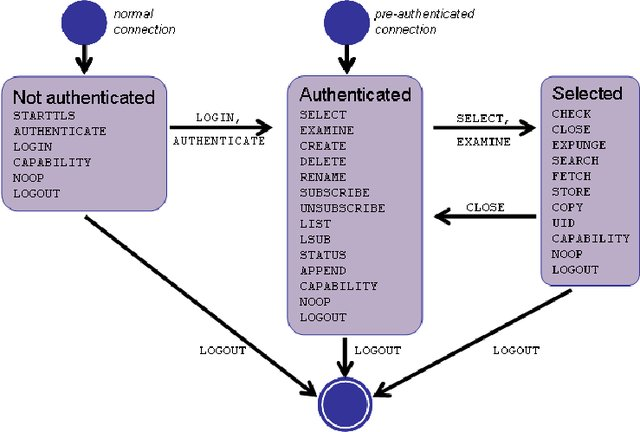
\includegraphics[width=8cm]{IMAP-protocol-finite-state-machine_W640}
\caption{IMAP State Machine}
\end{figure}

\item HTTP | Gmail, Hotmail, etc
\end{itemize}
\newpage
\item Explain the purpose of each POP command and the meanings of the response codes
\begin{figure}[!h]
\centering
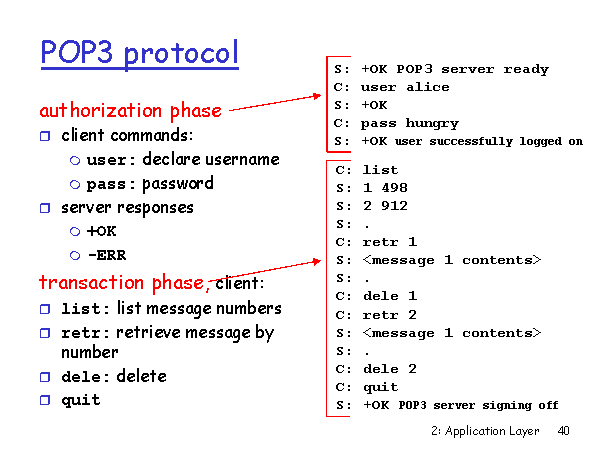
\includegraphics[width=10cm]{POP3_Commands}
\caption{POP3 Command Sequence}
\end{figure}
\begin{itemize}
\item Please refer to \href{https://www.shellhacks.com/retrieve-email-pop3-server-command-line/}{\underline{here}} for more information about commands for POP3
\end{itemize}

\item In POP protocol, what is the difference between download-and-keep and download-and-delete?
\begin{itemize}
\item \textbf{Download-and-keep:} UA leaves copies of messages on mail server after downloading
\item \textbf{Download-and-delete:} UA deletes copies of messages on mail server after downloading
\end{itemize}

\item What is the difference between POP and IMAP
\begin{itemize}
\item POP is a stateless protocol. Only allows for pulling emails from a centralized server. After the pull, messages are discarded.
\item IMAP is a stateful protocol. Can provide an interface to a email file system.
\end{itemize}
\end{enumerate}

\end{document}

